\documentclass[journal,12pt,twocolumn]{IEEEtran}
%
\usepackage{setspace}
\usepackage{gensymb}
\usepackage{xcolor}
\usepackage{caption}
%\usepackage{subcaption}
%\doublespacing
\singlespacing

%\usepackage{graphicx}
%\usepackage{amssymb}
%\usepackage{relsize}
\usepackage[cmex10]{amsmath}
\usepackage{mathtools}
%\usepackage{amsthm}
%\interdisplaylinepenalty=2500
%\savesymbol{iint}
%\usepackage{txfonts}
%\restoresymbol{TXF}{iint}
%\usepackage{wasysym}
\usepackage{hyperref}
\usepackage{amsthm}
\usepackage{mathrsfs}
\usepackage{txfonts}
\usepackage{stfloats}
\usepackage{cite}
\usepackage{cases}
\usepackage{subfig}
%\usepackage{xtab}
\usepackage{longtable}
\usepackage{multirow}
%\usepackage{algorithm}
%\usepackage{algpseudocode}
%\usepackage{enumerate}
\usepackage{enumitem}
\usepackage{mathtools}
%\usepackage{iithtlc}
%\usepackage[framemethod=tikz]{mdframed}
\usepackage{listings}
\usepackage{scalerel}
\usepackage{stackengine}
\usepackage{xcolor}
\newcommand\showdiv[1]{\overline{\smash{\hstretch{.5}{)}\mkern-3.2mu\hstretch{.5}{)}}#1}}
\usepackage{polynom}
%\usepackage{stmaryrd}
\let\vec\mathbf

%\usepackage{wasysym}
%\newcounter{MYtempeqncnt}
\DeclareMathOperator*{\Res}{Res}
%\renewcommand{\baselinestretch}{2}
\renewcommand\thesection{\arabic{section}}
\renewcommand\thesubsection{\thesection.\arabic{subsection}}
\renewcommand\thesubsubsection{\thesubsection.\arabic{subsubsection}}

\renewcommand\thesectiondis{\arabic{section}}
\renewcommand\thesubsectiondis{\thesectiondis.\arabic{subsection}}
\renewcommand\thesubsubsectiondis{\thesubsectiondis.\arabic{subsubsection}}

%\renewcommand{\labelenumi}{\textbf{\theenumi}}
%\renewcommand{\theenumi}{P.\arabic{enumi}}

% correct bad hyphenation here
\hyphenation{op-tical net-works semi-conduc-tor}

\lstset{
	language=Python,
	frame=single, 
	breaklines=true,
	columns=fullflexible
}



\begin{document}
	%
	
	\theoremstyle{definition}
	\newtheorem{theorem}{Theorem}[section]
	\newtheorem{problem}{Problem}
	\newtheorem{proposition}{Proposition}[section]
	\newtheorem{lemma}{Lemma}[section]
	\newtheorem{corollary}[theorem]{Corollary}
	\newtheorem{example}{Example}[section]
	\newtheorem{definition}{Definition}[section]
	%\newtheorem{algorithm}{Algorithm}[section]
	%\newtheorem{cor}{Corollary}
	\newcommand{\BEQA}{\begin{eqnarray}}
		\newcommand{\EEQA}{\end{eqnarray}}
	\newcommand{\define}{\stackrel{\triangle}{=}}
	\newcommand{\myvec}[1]{\ensuremath{\begin{pmatrix}#1\end{pmatrix}}}
	\newcommand{\mydet}[1]{\ensuremath{\begin{vmatrix}#1\end{vmatrix}}}
	
	
	\bibliographystyle{IEEEtran}
	%\bibliographystyle{ieeetr}
	
	\providecommand{\nCr}[2]{\,^{#1}C_{#2}} % nCr
	\providecommand{\nPr}[2]{\,^{#1}P_{#2}} % nPr
	\providecommand{\mbf}{\mathbf}
	\providecommand{\pr}[1]{\ensuremath{\Pr\left(#1\right)}}
	\providecommand{\qfunc}[1]{\ensuremath{Q\left(#1\right)}}
	\providecommand{\sbrak}[1]{\ensuremath{{}\left[#1\right]}}
	\providecommand{\lsbrak}[1]{\ensuremath{{}\left[#1\right.}}
	\providecommand{\rsbrak}[1]{\ensuremath{{}\left.#1\right]}}
	\providecommand{\brak}[1]{\ensuremath{\left(#1\right)}}
	\providecommand{\lbrak}[1]{\ensuremath{\left(#1\right.}}
	\providecommand{\rbrak}[1]{\ensuremath{\left.#1\right)}}
	\providecommand{\cbrak}[1]{\ensuremath{\left\{#1\right\}}}
	\providecommand{\lcbrak}[1]{\ensuremath{\left\{#1\right.}}
	\providecommand{\rcbrak}[1]{\ensuremath{\left.#1\right\}}}
	\theoremstyle{remark}
	\newtheorem{rem}{Remark}
	\newcommand{\sgn}{\mathop{\mathrm{sgn}}}
	
	\providecommand{\abs}[1]{\left\vert#1\right\vert}
	\providecommand{\res}[1]{\Res\displaylimits_{#1}} 
	\providecommand{\norm}[1]{\lVert#1\rVert}
	\providecommand{\mtx}[1]{\mathbf{#1}}
	\providecommand{\mean}[1]{E\left[ #1 \right]}
	\providecommand{\fourier}{\overset{\mathcal{F}}{ \rightleftharpoons}}
	\providecommand{\ztrans}{\overset{\mathcal{Z}}{ \rightleftharpoons}}

	%\providecommand{\hilbert}{\overset{\mathcal{H}}{ \rightleftharpoons}}
	\providecommand{\system}{\overset{\mathcal{H}}{ \longleftrightarrow}}
	%\newcommand{\solution}[2]{\textbf{Solution:}{#1}}
	\newcommand{\solution}{\noindent \textbf{Solution: }}
	\providecommand{\dec}[2]{\ensuremath{\overset{#1}{\underset{#2}{\gtrless}}}}
	\numberwithin{equation}{section}
	%\numberwithin{equation}{subsection}
	%\numberwithin{problem}{subsection}
	%\numberwithin{definition}{subsection}
	\makeatletter
	\@addtoreset{figure}{problem}
	\makeatother
	
	\let\StandardTheFigure\thefigure
	%\renewcommand{\thefigure}{\theproblem.\arabic{figure}}
	\renewcommand{\thefigure}{\theproblem}
	
	
	%\numberwithin{figure}{subsection}
	
	\def\putbox#1#2#3{\makebox[0in][l]{\makebox[#1][l]{}\raisebox{\baselineskip}[0in][0in]{\raisebox{#2}[0in][0in]{#3}}}}
	\def\rightbox#1{\makebox[0in][r]{#1}}
	\def\centbox#1{\makebox[0in]{#1}}
	\def\topbox#1{\raisebox{-\baselineskip}[0in][0in]{#1}}
	\def\midbox#1{\raisebox{-0.5\baselineskip}[0in][0in]{#1}}
	
	\vspace{3cm}
	
	\title{ EE 3900 - Assignment 1}
	
	\author{VIBHAVASU}
	
	% make the title area
	\maketitle
	
	%\newpage
	
	\tableofcontents
	
	%\renewcommand{\thefigure}{\thesection.\theenumi}
	%\renewcommand{\thetable}{\thesection.\theenumi}
	
	\renewcommand{\thefigure}{\theenumi}
	\renewcommand{\thetable}{\theenumi}
	
	%\renewcommand{\theequation}{\thesection}
	
	
	\bigskip
	
	\begin{abstract}
		This manual provides a simple introduction to digital signal processing.
	\end{abstract}
	\section{Software Installation}
	Run the following commands
	\begin{lstlisting}
sudo apt-get update
sudo apt-get install libffi-dev libsndfile1 python3-scipy  python3-numpy python3-matplotlib 
sudo pip install cffi pysoundfile 
	\end{lstlisting}
	\section{Digital Filter}
	\begin{enumerate}[label=\thesection.\arabic*
		,ref=\thesection.\theenumi]
		\item
		\label{prob:input}
		Download the sound file from  
		\begin{lstlisting}
wget https://raw.githubusercontent.com/gadepall/EE1310/master/filter/codes/Sound_Noise.wav
		\end{lstlisting}
		%\href{http://tlc.iith.ac.in/img/sound/Sound_Noise.wav}{\url{http://tlc.iith.ac.in/img/sound/Sound_Noise.wav}}  
		%in the link given below.
		%\linebreak
		\item
		\label{prob:spectrogram}
		You will find a spectrogram at \href{https://academo.org/demos/spectrum-analyzer}{\url{https://academo.org/demos/spectrum-analyzer} }. 
		%\end{problem}
		%%
		%
		%%\onecolumn
		%%\input{./figs/fir}
		%\begin{problem}
		Upload the sound file that you downloaded in Problem \ref{prob:input} in the spectrogram  and play.  Observe the spectrogram. What do you find?
		\\
		%
		\solution There are a lot of yellow lines between 440 Hz to 5.1 KHz.  These represent the synthesizer key tones. Also, the key strokes
		are audible along with background noise.
		% By observing spectrogram, it clearly shows that tonal frequency is under 4kHz. And above 4kHz only noise is present.
		\item
		\label{prob:output}
		Write the python code for removal of out of band noise and execute the code.
		\\
		\solution
		\lstinputlisting{./codes/Cancel_noise.py}
		%\begin{figure}[h]
		%\centering
		%\includegraphics[width=\columnwidth]{enc_block_diag.png}
		%\caption{}
		%\label{fig:convolution encoder}
		%\end{figure}
		%\input{block_enc}
		\item
		The output of the python script in Problem \ref{prob:output} is the audio file Sound\_With\_ReducedNoise.wav. Play the file in the spectrogram in Problem \ref{prob:spectrogram}. What do you observe?
		\\
		\solution The key strokes as well as background noise is subdued in the audio.  Also,  the signal is blank for frequencies above 5.1 kHz.
		
	\end{enumerate}
	\section{Difference Equation}
	\begin{enumerate}[label=\thesection.\arabic*,ref=\thesection.\theenumi]
		\item Let
		\begin{equation}
			\label{def:xn}
			x(n) = \cbrak{\underset{\uparrow}{1},2,3,4,2,1}
		\end{equation}
		Sketch $x(n)$.
		\item Let
		\begin{multline}
			\label{eq:iir_filter}
			y(n) + \frac{1}{2}y(n-1) = x(n) + x(n-2), 
			\\
			y(n) = 0, n < 0
		\end{multline}
		Sketch $y(n)$.
		\\
		\solution The following code yields Fig. \ref{fig:xnyn}.
		\begin{lstlisting}
wget https://github.com/gadepall/EE1310/raw/master/filter/codes/xnyn.py
		\end{lstlisting}
		\begin{figure}[!ht]
			\begin{center}
				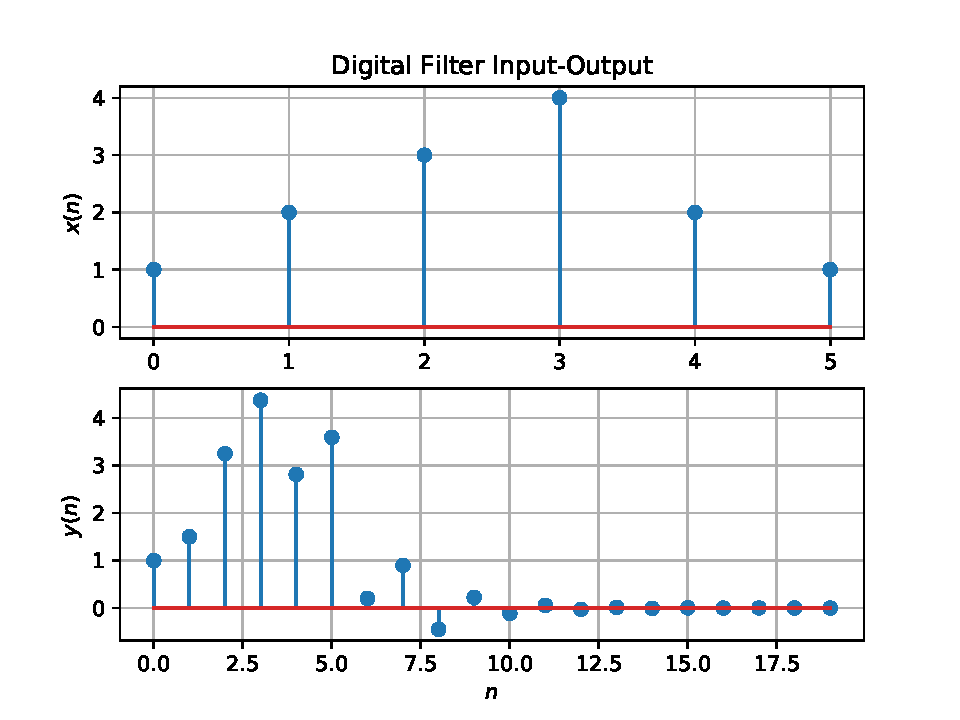
\includegraphics[width=\columnwidth]{./figs/xnyn}
			\end{center}
			\captionof{figure}{}
			\label{fig:xnyn}	
		\end{figure}
		
		\item Repeat the above exercise using a C code.
		\solution: C Code
		\begin{lstlisting}
wget https://github.com/DarkWake9/EE3900/blob/main/Assignment%201/e3-3.c
		\end{lstlisting}
		\solution: Python Code
\begin{lstlisting}
wget https://github.com/DarkWake9/EE3900/blob/main/Assignment%201/e3-3.py
\end{lstlisting}		
	\end{enumerate}
	\section{$Z$-transform}
	\begin{enumerate}[label=\thesection.\arabic*]
		\item The $Z$-transform of $x(n)$ is defined as
		%
		\begin{equation}
			\label{eq:z_trans}
			X(z)={\mathcal {Z}}\{x(n)\}=\sum _{n=-\infty }^{\infty }x(n)z^{-n}
		\end{equation}
		%
		Show that
		\begin{equation}
			\label{eq:shift1}
			{\mathcal {Z}}\{x(n-1)\} = z^{-1}X(z)
		\end{equation}
		and find
		\begin{equation}
			{\mathcal {Z}}\{x(n-k)\} 
		\end{equation}
		\solution From \eqref{eq:z_trans},
		\begin{align}
			{\mathcal {Z}}\{x(n-k)\} &=\sum _{n=-\infty }^{\infty }x(n-1)z^{-n}
			\\
			&=\sum _{n=-\infty }^{\infty }x(n)z^{-n-1} = z^{-1}\sum _{n=-\infty }^{\infty }x(n)z^{-n}
		\end{align}
		resulting in \eqref{eq:shift1}. Similarly, it can be shown that
		%
		\begin{equation}
			\label{eq:z_trans_shift}
			{\mathcal {Z}}\{x(n-k)\} = z^{-k}X(z)
		\end{equation}
		\item Obtain $X(z)$ for $x(n)$ defined in problem 
		\ref{def:xn}.
		\item Find
		%
		\begin{equation}
			H(z) = \frac{Y(z)}{X(z)}
		\end{equation}
		%
		from  \eqref{eq:iir_filter} assuming that the $Z$-transform is a linear operation.
		\\
		\solution  Applying \eqref{eq:z_trans_shift} in \eqref{eq:iir_filter},
		\begin{align}
			Y(z) + \frac{1}{2}z^{-1}Y(z) &= X(z)+z^{-2}X(z)
			\\
			\implies H(z) = \frac{Y(z)}{X(z)} &= \frac{1 + z^{-2}}{1 + \frac{1}{2}z^{-1}}
			\label{eq:freq_resp}
		\end{align}
		%
		\item 
		\begin{enumerate}
	
	\item Find the Z transform of 
		\begin{equation}
			\delta(n)
			=
			\begin{cases}
				1 & n = 0
				\\
				0 & \text{otherwise}
			\end{cases}
		\end{equation}
		\item and show that the $Z$-transform of
		\begin{equation}
			\label{eq:unit_step}
			u(n)
			=
			\begin{cases}
				1 & n \ge 0
				\\
				0 & \text{otherwise}
			\end{cases}
		\end{equation}
		is
		\begin{equation}
			U(z) = \frac{1}{1-z^{-1}}, \quad \abs{z} > 1
		\end{equation}
			\end{enumerate}
		\solution It is easy to show that
		\begin{equation}
			\delta(n) \ztrans 1
		\end{equation}
		and from \eqref{eq:unit_step},
		\begin{align}
			U(z) &= \sum _{n= 0}^{\infty}z^{-n}
			\\
			&=\frac{1}{1-z^{-1}}, \quad \abs{z} > 1
		\end{align}
		using the fomula for the sum of an infinite geometric progression.
		%
		\begin{enumerate}[label=(\roman*)]
			\item \solution \begin{equation}
				\Delta(z) = {\mathcal{Z}}\{\delta[n]\}=\sum_{n=-\infty}^{\infty} \delta(n) z^{-n} = 1\\
			\end{equation}
			
			\item \solution \begin{align}
				U(z) = {\mathcal{Z}}\{\delta(n)\}=\sum_{n=-\infty}^{\infty} u[n] z^{-n} \\
				=1+z^{-1}+z^{-2}+\cdots 
				=\frac{1}{1-z^{-1}}
			\end{align}
		\end{enumerate}
		
		\item Show that 
		\begin{equation}
			\label{eq:anun}
			a^nu(n) \ztrans \frac{1}{1-az^{-1}} \quad \abs{z} > \abs{a}
		\end{equation}
		
		\solution
		\begin{align}
			a^{n}u[n] = \begin{cases} a^{n} & n \geq 0 \\
				0 & n<0\end{cases} \\
			U^{\prime}(z)={\mathcal{Z}}\{a^{n}u[n]\}=\sum_{n=-\infty}^{\infty} a^{n}u[n] z^{-n}\\
			=1+az^{-1}+a^{2}z^{-2}+\cdots
		\end{align}
Given: $\abs{z} > \abs{a}$\\
		\begin{equation}
			\label{eq:U'} 
			U^{\prime}(z)=\frac{1}{1-a z^{-1}}
		\end{equation}
		\item Let
		\begin{equation}
			H\brak{e^{\j \omega}} = H\brak{z = e^{\j \omega}}.
		\end{equation}
		Plot $\abs{H\brak{e^{\j \omega}}}$.  Is it periodic? If so, find the period. $H(e^{\j \omega})$ is
		known as the {\em Discret Time Fourier Transform} (DTFT) of $h(n)$.\\
		\solution The following code plots Fig. $\ref{fig:dtft}$
		
		\begin{lstlisting}
wget https://raw.githubusercontent.com/gadepall/EE1310/master/filter/codes/dtft.py
		\end{lstlisting}
		\begin{figure}[!ht]
			\centering
			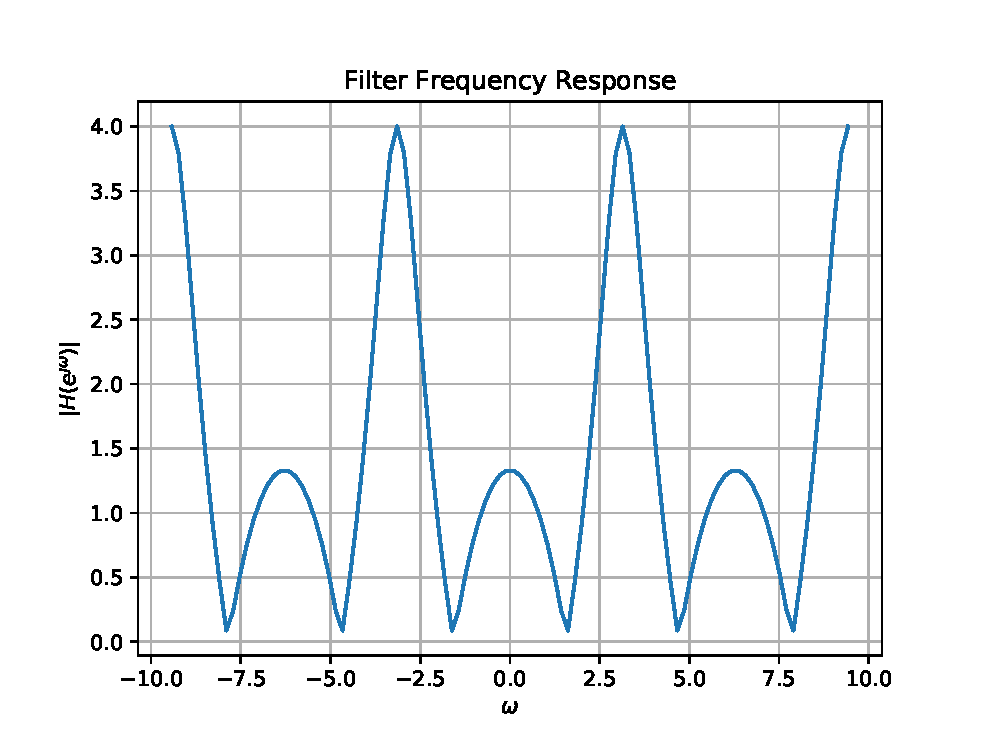
\includegraphics[width=\columnwidth]{./figs/dtft}
			\caption{$\abs{H\brak{e^{\j\omega}}}$}
\label{fig:dtft}
		\end{figure}
%	\raggedright{ \quad \quad $\therefore$ Period of $H(e^{\j \omega})$ is $2\pi$\\
\solution From \eqref{eq:freq_resp} we get
	\begin{align}
		%H\brak{e^{\j \omega}} = H\brak{z = e^{\j \omega}}\\
		H\brak{e^{\j \omega}}=\frac{1 + e^{-2\j \omega}}{1 + \frac{1}{2}e^{-\j \omega}}\\
		=\frac{e^{\j \omega} + e^{-\j \omega}}{e^{\j \omega} + \frac{1}{2}}
		=\frac{2\cos\brak{\omega}}{e^{\j \omega} + \frac{1}{2}}\\
		\implies \abs{H\brak{e^{\j \omega}}}\\
		=\frac{2\cos\omega}{\sqrt{\brak{\cos\omega+\frac{1}{2}}^{2}+\sin^2\omega}}
	\end{align}
	\begin{align}
		=\frac{2\cos\omega}{\sqrt{\cos^2\omega + \sin^2 \omega + \cos \omega + \frac{1}{4}}}\\
		=\frac{2\cos\omega}{\sqrt{\frac{5}{4}+\cos\omega}}
	\end{align}
	For a periodic function of period $T$,
	\begin{align}
		f\brak{x} = f\brak{x+T}, T \neq 0	 
	\end{align}

	Checking if $\pi$ is a period,

	\begin{align}
		\frac{2\cos\brak{\omega+\pi}}{\sqrt{\frac{5}{4}+\cos\brak{\omega+\pi}}}\\ =
		\frac{-2\cos\omega}{\sqrt{\frac{5}{4}-\cos\omega}}\\
		\implies H\brak{e^{\j \brak{\omega+\pi}}} \neq H\brak{e^{\j \omega}}\\
	\intertext{Checking if $2\pi$ is a period}
		\dfrac{2\cos\brak{\omega+2\pi}}{\sqrt{\frac{5}{4}+\cos\brak{\omega + 2\pi}}} =
		\frac{2\cos \omega}{\sqrt{\frac{5}{4} + \cos \omega }}\\
		\implies H\brak{e^{\j \brak{\omega + 2\pi}}} = H\brak{e^{\j \omega}}
	\end{align}
	
$\therefore$ Period of $H(e^{\j \omega})$ is $2\pi$\\
	\item Express $h(n)$ in terms of $H\brak{e^{\j \omega}}$ \\[5pt]
	\solution
		\begin{align}
		H( e^{j\omega }) =\sum ^{\infty }_{n=-\infty }h(n') e^{-j\omega n'}\\
		\implies \int_{\-\pi} ^{\pi }	H\left( e^{j\omega }\right) e^{j\omega n}d\omega\\			
		= \sum_{n'=-\infty }^{\infty } \int ^{\pi }_{-\pi }h(n') e^{-j\omega n'}e^{j\omega n}d\omega\\			
		=\sum ^{\infty }_{n'=-\infty }h(n') 2\pi \delta(n'- n) =
	 2\pi h(n) 
		\end{align}
	\begin{equation}
		\therefore	 h(n) =\dfrac{1}{2\pi }\int ^{\pi }_{-\pi }H\left( e^{j \omega}\right) e^{j\omega }d\omega 
	\end{equation}

	\end{enumerate}
	
	\section{Impulse Response}
	\begin{enumerate}[label=\thesection.\arabic*]
		\item Using long division, 
		find
		\begin{align}
			h(n), \quad n < 5
		\end{align}
		for H(z) in 
		\eqref{eq:freq_resp}.\\
		\solution
		from \eqref{eq:freq_resp}
		\begin{align}
			H(z) %= \frac{1 + z^{-2}}{1 + \frac{1}{2}z^{-1}}
			= (1 + z^{-2})\brak{1+\frac{1}{2}z^{-1}}^{-1}\\
			\text{For ROC:} \quad \abs{\frac{1}{2}z^{-1}} < 1\\
			\implies \abs{z} > \frac{1}{2} \text{ is the ROC for this case}
			\end{align}
	\tiny
		\begin{align*}
			&\underline{1-\dfrac{1}{2}z^{-1}+\dfrac{5}{4}z^{-2}-\dfrac{5}{8}z^{-3}+\frac{5}{16}z^{-4}}\ldots \ldots\\
			\rbrak{1 + \dfrac{1}{2}z^{-1}} &\text{\quad}\text{\quad}\text{\quad}\text{   }\text{$1 + z^{-2}$}\\
			&\text{\quad}\text{\quad}\text{\quad}\underline{\text{ }1 + \frac{1}{2}z^{-1}}\\
			&\text{\quad}\text{\quad}\text{\quad}\text{ }\text{ }\text{ }-\frac{z^{-1}}{2}+z^{-2}\\
			&\text{\quad}\text{\quad}\text{\quad}\text{ }\text{ }\underline{\text{} -\frac{z^{-1}}{2} - \frac{1}{4}z^{-2}}\\
			&\text{\quad}\text{\quad}\text{\quad}\text{ }\text{ }\underline{\text{ }\text{ }\text{ }\text{ }\frac{5}{4}z^{-2}\text{\quad \quad \quad \quad}}\\
			&\text{\quad}\text{\quad}\text{\quad}\text{ }\text{ }\underline{\text{ }\text{ }\text{ }\text{ }\frac{5}{4}z^{-2} + \frac{5}{8}z^{-3}}\\
			&\text{\quad}\text{\quad}\text{\quad}\text{ }\text{ }\underline{\text{ }\text{ }\text{ }\text{\quad}-\frac{5}{8}z^{-3}\text{\quad}\text{\quad}}\\
			&\text{\quad}\text{\quad}\text{\quad}\text{ }\text{ }\underline{\text{ }\text{ }\text{ }\text{ }\text{ }-\frac{5}{8}z^{-3} - \frac{5}{16}z^{-4}}\\
			&\text{\quad}\text{\quad}\text{\quad}\text{ }\text{ }\underline{\text{ }\text{ }\text{ }\text{ }\text{ }\text{\quad}\frac{5}{16}z^{-4}\text{\quad}\text{\quad}}\\
			&\text{\quad}\text{\quad}\text{\quad}\text{ }\text{ }\text{ }\text{ }\text{ }\text{ }\text{ }\frac{5}{16}z^{-4} + \frac{5}{32}z^{-5}\\
			&\text{\quad}\text{\quad}\text{\quad}\text{\quad}\text{\quad}\text{\quad}\text{\quad} \normalsize \vdots
		\end{align*}
	\normalsize
		\begin{align}
			\implies H(z) = \frac{1 + z^{-2}}{1+\tfrac{1}{2}z^{-1}} = 1 - \tfrac{1}{2}z^{-1} + \sum_{n=2}^{\infty}\frac{5}{4}z^{-n}\\
			\text{We know that } H(z) =\sum ^{\infty }_{n=-\infty }h(n) z^{-n}\\
			\intertext{comparing coefficients: \($ in the ROC $\abs{z} > \frac{1}{2}\)}
			h(n) = \begin{cases}
				%\doublespacing
				0 \quad $if \quad$ n < 0\\
				1, \quad $if \quad$ n = 0\\
				-\frac{1}{2}$, \quad if \quad$ n = 1\\
				5\brak{-\tfrac{1}{2}}^{n}$, \quad if \quad$ n \ge 2
			\end{cases}\\
			h(0) = 1$,\quad$ h(1) = -\frac{1}{2}$,\quad$ h(2) = \tfrac{5}{4}\\
			h(3) = -\tfrac{5}{8}$,\quad$ h(4) = \tfrac{5}{16}
		\end{align}
		\item \label{prob:impulse_resp}
		Find an expression for $h(n)$ using $H(z)$, given that 
		%in Problem \ref{eq:ztransab} and \eqref{eq:anun}, given that
		\begin{equation}
			\label{eq:impulse_resp}
			h(n) \ztrans H(z)
		\end{equation}
		and there is a one to one relationship between $h(n)$ and $H(z)$. $h(n)$ is known as the {\em impulse response} of the
		system defined by \eqref{eq:iir_filter}.
		\\
		\solution From \eqref{eq:freq_resp},
		\begin{align}
			H(z) &= \frac{1}{1 + \frac{1}{2}z^{-1}} + \frac{ z^{-2}}{1 + \frac{1}{2}z^{-1}}
			\\
			\therefore h(n) &= \brak{-\frac{1}{2}}^{n}u(n) + \brak{-\frac{1}{2}}^{n-2}u(n-2)
		\end{align}
		using \eqref{eq:anun} and \eqref{eq:z_trans_shift}.
		\item Sketch $h(n)$. Is it bounded? Justify theoretically.
		\\
		\solution The following code plots Fig. \ref{fig:hn}.
		\begin{lstlisting}
wget https://raw.githubusercontent.com/gadepall/EE1310/master/filter/codes/hn.py
		\end{lstlisting}
		\begin{figure}[!ht]
			\centering
			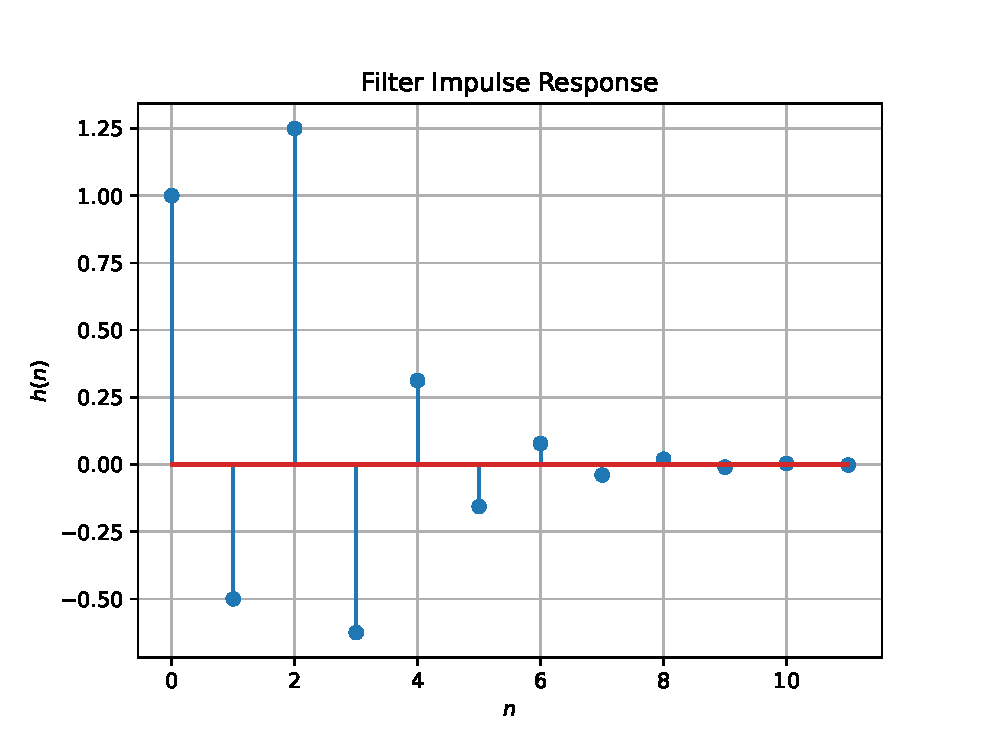
\includegraphics[width=0.9\columnwidth]{./figs/hn}
			\caption{$h(n)$ as the inverse of $H(z)$}
			\label{fig:hn}
		\end{figure}
%	\vspace{7.5cm}
		\item Convergent? Justify using the ratio test.\\
		\solution\\
		\begin{align}
			\onehalfspacing
			h(n) = \begin{cases}
				\doublespacing
				0 \quad $if \quad$ n < 0\\
				1, \quad $if \quad$ n = 0\\
				-\frac{1}{2}$, \quad if \quad$ n = 1\\
				5\brak{-\tfrac{1}{2}}^{n}$, \quad if \quad$ n \ge 2
			\end{cases}\\
		\intertext{Using ratio test:}
		\lim_{n \rightarrow \infty} \abs{\dfrac{h(n+1)}{h(n)}} = \abs{\dfrac{5\brak{-\tfrac{1}{2}}^{n+1}}{5\brak{-\tfrac{1}{2}}^{n}}}
		= \frac{1}{2} < \infty
		\end{align}
\singlespacing
		$\implies h(n)$ is convergent\\
		\item The system with $h(n)$ is defined to be stable if
		\begin{equation}
			\sum_{n=-\infty}^{\infty}h(n) < \infty
		\end{equation}
		Is the system defined by \eqref{eq:iir_filter} stable for the impulse response in \eqref{eq:impulse_resp}\\
		\solution
		\begin{align}
			\sum_{n=-\infty}^{\infty}h(n) = 0 + 1 - \frac{1}{2} + 5\sum_{n=2}^{\infty} \brak{-\dfrac{1}{2}}^{n}\\
			= \dfrac{1}{2} + 5\brak{1 - \dfrac{1}{2} - \brak{\dfrac{1}{1 + \tfrac{1}{2}}}}\\
			= \dfrac{1}{2} + \dfrac{5}{6} = \dfrac{8}{6} = 1.333 < \infty
		\end{align}
			$\therefore h(n)$  is Stable\\
		\item Verify the above result using a python code.\\
		\solution The Following code computes and proves the aboves result
		\begin{lstlisting}
wget https://github.com/DarkWake9/EE3900/blob/main/Assignment%201/e5-6.py
		\end{lstlisting}
		\item 
		Compute and sketch $h(n)$ using 
		\begin{equation}
			\label{eq:iir_filter_h}
			h(n) + \frac{1}{2}h(n-1) = \delta(n) + \delta(n-2), 
		\end{equation}
		%
		This is the definition of $h(n)$.
		\\\\
		\solution The following code plots Fig. \ref{fig:hndef}. Note that this is the same as Fig. \ref{fig:hn}. \\\\
		\begin{lstlisting}
wget https://raw.githubusercontent.com/gadepall/EE1310/master/filter/codes/hndef.py
		\end{lstlisting}
		\begin{figure}[!ht]
			\centering
			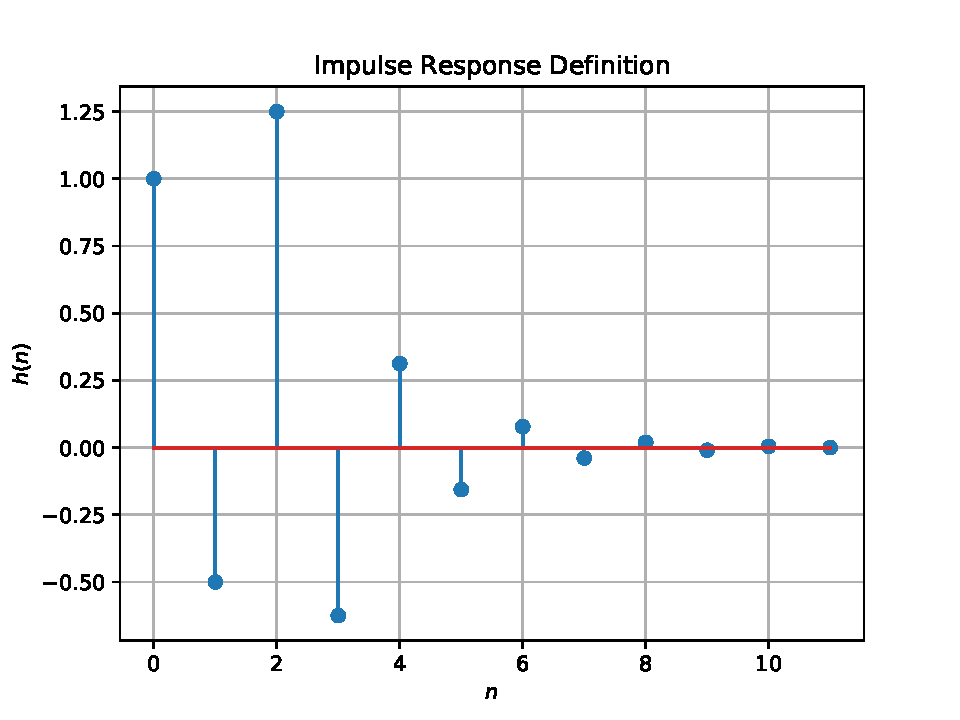
\includegraphics[width=\columnwidth]{./figs/hndef}
			\caption{$h(n)$ from the definition}
			\label{fig:hndef}
		\end{figure}
%		\\[100pt]
		\item Compute 
		%
		\begin{equation}
			\label{eq:convolution}
			y(n) = x(n)*h(n) = \sum_{n=-\infty}^{\infty}x(k)h(n-k)
		\end{equation}
		
		Comment. The operation in \eqref{eq:convolution} is known as
		{\em convolution}.
		
		\solution The following code plots Fig. \ref{fig:ynconv}. Note that this is the same as 
		$y(n)$ in  Fig. 
		\ref{fig:xnyn}. 
		%
		\begin{lstlisting}
wget https://raw.githubusercontent.com/gadepall/EE1310/master/filter/codes/ynconv.py
		\end{lstlisting}
		\begin{figure}[!ht]
			\centering
			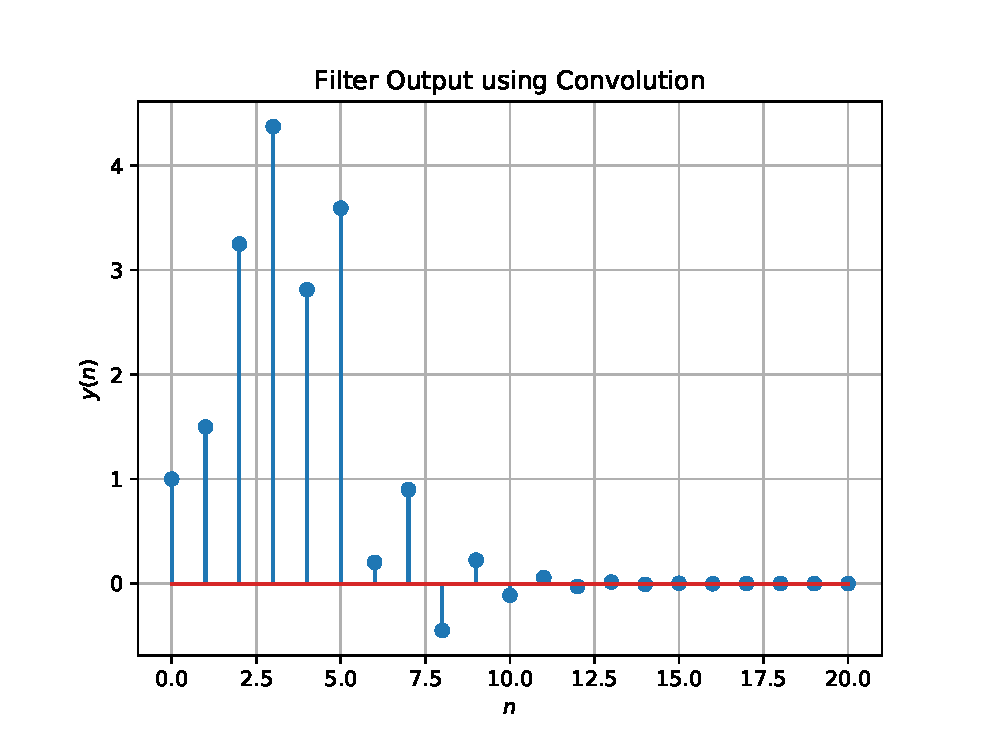
\includegraphics[width=\columnwidth]{./figs/ynconv}
			\caption{\small $y(n)$ from the definition of convolution}
			\label{fig:ynconv}
		\end{figure}
	\vspace{5cm}
		\item Express the above convolution using a Teoplitz matrix.\\
		\solution From \eqref{def:xn}
				$x(n) = \cbrak{1,2,3,4,2,1}$\\
			From \eqref{eq:convolution}	$y(n) = x(n)*h(n)$\\
%			n = 0, $\ldots$ 6\\
			\begin{equation}
			\scriptsize 
			\left(
			\begin{smallmatrix}
				x(1) & 0 & 0 & 0 & 0 & 0 & 0 & 0 & 0 & 0 & 0 & 0\\
				x(2) & x(1) & 0 &0 & 0 & 0 & 0 & 0 &  0 & 0 & 0 & 0\\
				x(3) & x(2) & x(1) & 0 & 0 & 0 & 0 &  0 & 0 & 0 & 0 & 0\\
				x(4) & x(3) & x(2) & x(1) & 0 & 0 & 0 & 0 & 0 & 0 & 0 & 0\\
				x(5) & x(4) & x(3) & x(2)&x(1) & 0 & 0 & 0 & 0 & 0 & 0 & 0\\
				x(6) & x(5) & x(4) & x(3)&x(2)&x(1)&0&0&0&0&0&0\\
				0 & x(6) & x(5) & x(4)&x(3)&x(2)&x(1)&0&0&0&0&0\\
				0 & 0 & x(6) & x(5)& x(4)&x(3)&x(2)&x(1)&0&0&0&0\\
				0 & 0 & 0 & x(6) & x(5)&x(4)&x(3)&x(2)&x(1)&0&0&0\\
				0 & 0 & 0 & 0 & x(6) & x(5)&x(4)&x(3)&x(2)&x(1)&0&0\\
				0 & 0 & 0 & 0 & 0 & x(6)&x(5)&x(4)&x(3)&x(2)&x(1)&0\\
				0 & 0 & 0 & 0 & 0 & 0 &x(6)&x(5)&x(4)&x(3)&x(2)&x(1)\\
				0 & 0 & 0 & 0 & 0 & 0 & 0 & x(6)&x(5)&x(4)&x(3)&x(2)\\
				0 & 0 & 0 & 0 & 0 & 0 & 0 & 0 &x(6)&x(5)&x(4)&x(3)\\
				0 & 0 & 0 & 0 & 0 & 0 & 0 & 0 & 0 &x(6)&x(5)&x(4)\\
				0 & 0 & 0 & 0 & 0 & 0 & 0 & 0 & 0 & 0 &x(6)&x(5)\\
				0 & 0 & 0 & 0 & 0 & 0 & 0 & 0 & 0 & 0 & 0 &x(6)\\
				0 & 0 & 0 & 0 & 0 & 0 & 0 & 0 & 0 & 0 & 0 & 0\\
			\end{smallmatrix}
					\right)
						\left(
			\begin{smallmatrix}
				h(1)\\h(2)\\h(3)\\h(4)\\h(5)\\h(6)\\h(7)\\h(8)\\h(9)\\h(10)\\h(11)\\h(12)
			\end{smallmatrix}
			\right)	
		\normalsize
			\end{equation}	
		\begin{align}
			\left(	\begin{smallmatrix}
				1&0&0&0&0&0&0&0&0&0&0&0\\
				2&1&0&0&0&0&0&0&0&0&0&0\\
				3&2&1&0&0&0&0&0&0&0&0&0\\
				4&3&2&1&0&0&0&0&0&0&0&0\\
				2&4&3&2&1&0&0&0&0&0&0&0\\
				1&2&4&3&2&1&0&0&0&0&0&0\\
				0&1&2&4&3&2&1&0&0&0&0&0\\
				0&0&1&2&4&3&2&1&0&0&0&0\\
				0&0&0&1&2&4&3&2&1&0&0&0\\
				0&0&0&0&1&2&4&3&2&1&0&0\\
				0&0&0&0&0&1&2&4&3&2&1&0\\
				0&0&0&0&0&0&1&2&4&3&2&1\\
				0&0&0&0&0&0&0&1&2&4&3&2\\
				0&0&0&0&0&0&0&0&1&2&4&3\\
				0&0&0&0&0&0&0&0&0&1&2&4\\
				0&0&0&0&0&0&0&0&0&0&1&2\\
				0&0&0&0&0&0&0&0&0&0&0&1\\
				0&0&0&0&0&0&0&0&0&0&0&0\\
			\end{smallmatrix} \right)
		\left(\begin{smallmatrix}1.   \\      -0.5    \\     1.25   \\    -0.625   \\    0.3125  \\   -0.15625 \\ 0.078125  \\  -0.0390625 \\  0.01953125 \\ -0.00976562 \\ 0.00390625 \\ -0.00195312
		\end{smallmatrix} \right)\\
		= \left(\begin{smallmatrix}
					1 \\ 1.5 \\ 3.25\\ 4.375\\
					2.8125 \\ 3.59375 \\ 0.203125 \\ 0.8984375\\
					-0.44921875 \\ 0.224609375 \\-0.112304688 \\ 0.0561523438\\
					-0.0280761719 \\ 0.0140380859 \\-7.01904297  \times 10^{-3} \\ 3.50952148 \times 10^{-3}\\
					-1.75476074 \times 10^{-3} \\ 8.77380371  \times 10^{-4} \\-4.38690186 \times 10^{-4} \\\\ 0 \\\\
		\end{smallmatrix}\right)
		\end{align}		
		\item Show that
		\begin{equation}
			y(n) =  \sum_{n=-\infty}^{\infty}x(n-k)h(k)
		\end{equation}
		\solution
		\begin{align}
			X(z) = {\mathcal{Z}} \{x(n)\}=\sum_{n=-\infty}^{\infty} x(n) z^{-n} \\
			H(z) = {\mathcal{Z}} \{h(m)\}=\sum_{m=-\infty}^{\infty} h(m) z^{-m} \\
			Y(z) = {\mathcal{Z}} \{h(m)\}=\sum_{k=-\infty}^{\infty} y(m) z^{-k}
		\end{align}
		
		\begin{equation}
			X(z)H(z)=\sum_{n=-\infty}^{\infty} x(n) z^{-n} \sum_{m=-\infty}^{\infty} h(m) z^{-m}
		\end{equation}
		\begin{align}
			=\sum_{n=-\infty}^{\infty} \sum_{m=-\infty}^{\infty} x[n] h[m] z^{-(n+m)} \\
			\intertext{Let $m = k - n$}
			=\sum_{k=-\infty}^{\infty}\left(\sum_{n=-\infty}^{\infty} x[n] h[n-k]\right) z^{-k} \\
			=\sum_{k=-\infty}^{\infty} y[n] z^{-k}=Y($z$) \\
			\implies Y(z) = X(z) \cdot H(z)
		\end{align}
		now put $n+m=k \quad n=-\infty$
		\begin{align}
			\Rightarrow Y(z)=\sum_{k=-\infty}^{\infty} x(m-k) \sum_{m=-\infty}^{\infty} h(m) z^{-k} \\
			=\sum_{k=-\infty}^{\infty}\left(\sum_{m=-\infty}^{\infty} x[m-k] h[k]\right) z^{-k} \\
			\text { but } Y(z)=\sum_{k=-\infty}^{\infty} y(m) z^{-k} \\
			\Rightarrow y(m)=\sum_{m=-\infty}^{\infty} x[m-k] h(k) \\
			\implies y(n)=\sum_{n=-\infty}^{\infty} x(n-k) h(k) 
		\end{align}
		
	\end{enumerate}
	
\section{DFT and FFT}
\begin{enumerate}[label=\thesection.\arabic*]
	\item
	Compute
	\begin{equation}
		X(k) \define \sum _{n=0}^{N-1}x(n) e^{-\j2\pi kn/N}, \quad k = 0,1,\dots, N-1
	\end{equation}
	and $H(k)$ using $h(n)$.\\
\newline	\solution
	\begin{figure}[!ht]
		\centering
		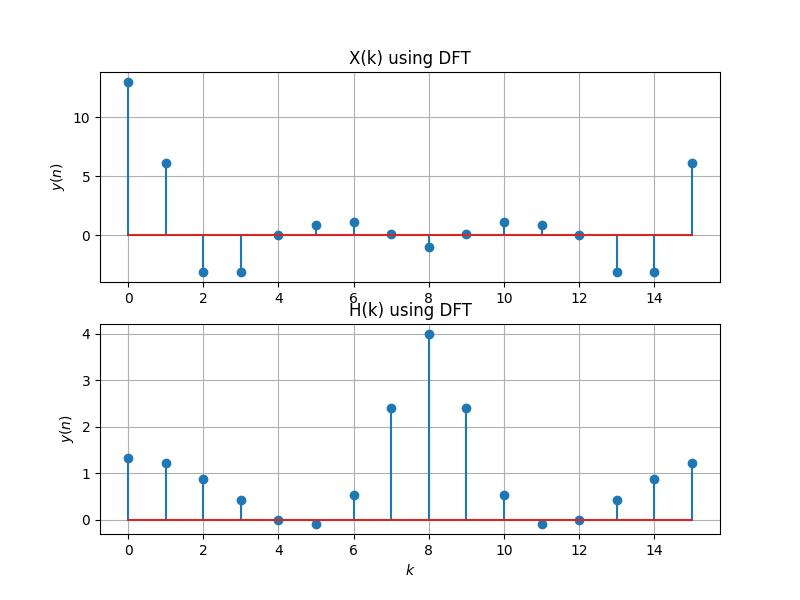
\includegraphics[width=\columnwidth]{./figs/e6.1DFT.jpg}
		\caption{$X(k)$ and $H(k)$ using DFT}
		\label{fig:Xkdft}
	\end{figure}
	\item Compute 
	\begin{equation}
		Y(k) = X(k)H(k)
	\end{equation}
	\solution
	\begin{figure}[!ht]
		\centering
		\includegraphics[width=\columnwidth]{./figs/XkDFT.jpg}
		\caption{$Y(k)$ using DFT}
		\label{fig:Ykdft}
	\end{figure}
	\item Compute
	\begin{equation}
		y\brak{n}={\frac {1}{N}}\sum _{k=0}^{N-1}Y\brak{k}\cdot e^{\j 2\pi kn/N},\quad n = 0,1,\dots, N-1
	\end{equation}
	\\
	\solution The following code plots Fig. \ref{fig:ynconv}. Note that this is the same as 
	$y(n)$ in  Fig. 
	\ref{fig:xnyn}. 
	%
	\begin{lstlisting}
wget https://raw.githubusercontent.com/gadepall/EE1310/master/filter/codes/yndft.py
	\end{lstlisting}
	\begin{figure}[!ht]
		\centering
		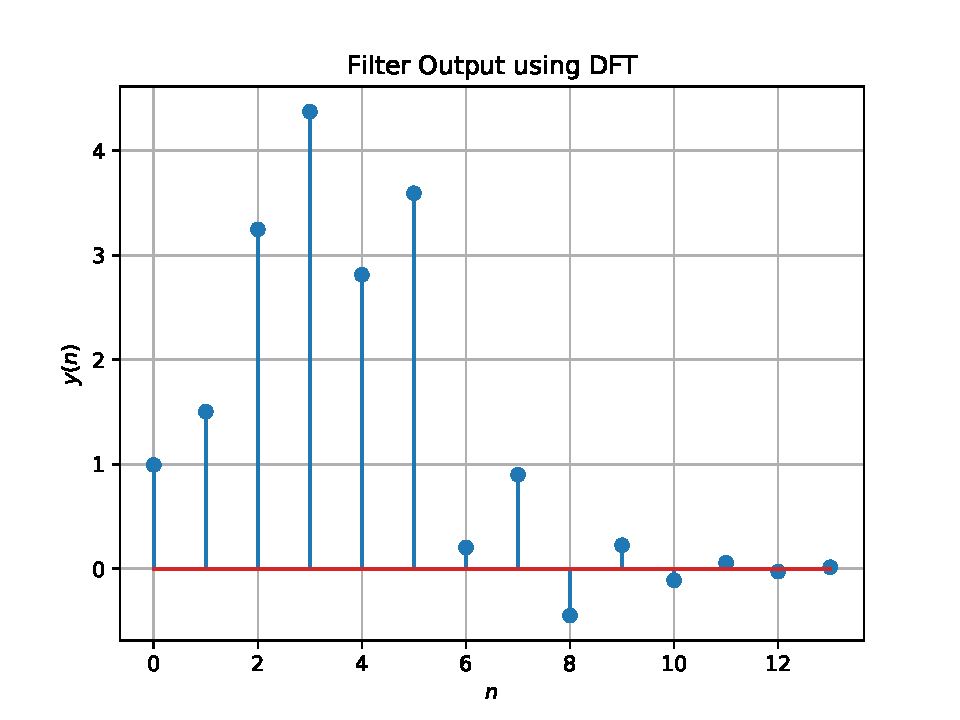
\includegraphics[width=\columnwidth]{./figs/yndft}
		\caption{$y(n)$ from the DFT}
		\label{fig:yndft}
	\end{figure}
	\item Repeat the previous exercise by computing $X(k), H(k)$ and $y(n)$ through FFT and 
	IFFT.
	\solution The following code plots Fig. \ref{fig:fft}, and \ref{fig:ifft}. 
	\begin{lstlisting}
wget https://github.com/DarkWake9/EE3900/blob/main/Assignment%201/e6.4.py
	\end{lstlisting}
	\begin{figure}[!ht]
		\centering
		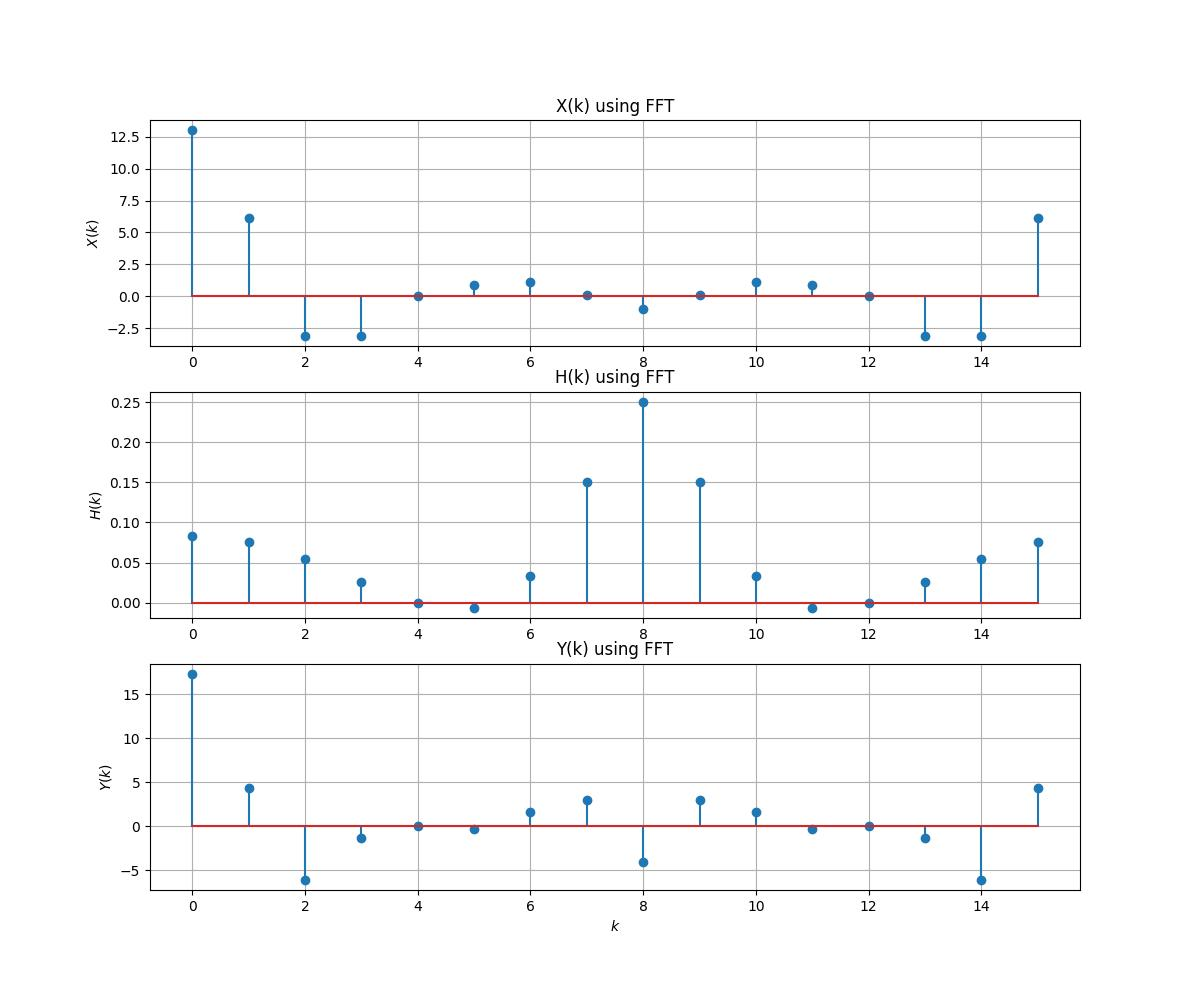
\includegraphics[width=\columnwidth]{./figs/e6.4-FFT.jpg}
		\caption{$X(k)$, $Y(k)$ and $H(k)$ using FFT}
		\label{fig:fft}
	\end{figure}
%	\vspace{5cm}
	\begin{figure}[!ht]
	\centering
	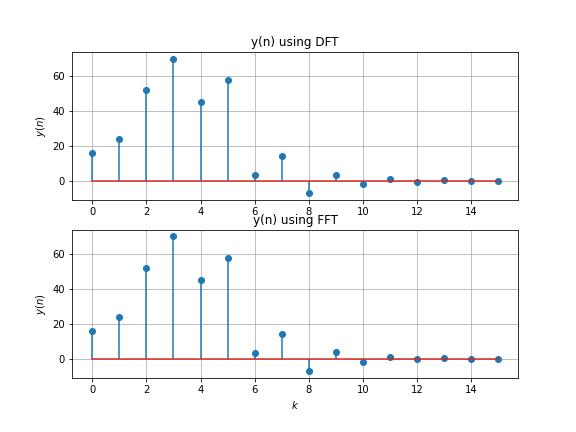
\includegraphics[width=\columnwidth]{./figs/e6.4DFT-FFT.jpg}
	\caption{Comparision of $y(n)$ obtained from \\ DFT (above) and IFFT (below)}
	\label{fig:dftfft}
	\end{figure}
	\end{enumerate}
	
\section{FFT}
% \subsection{Definitions}
\begin{enumerate}[label=\arabic*.,ref=\thesection.\theenumi]
	\numberwithin{equation}{section}
	\item The DFT of $x(n)$ is given by
\begin{align}
	X(k) \triangleq \sum_{n=0}^{N-1} x(n) e^{-j 2 \pi k n / N}, \quad k=0,1, \ldots, N-1
\end{align}
\item Let 
\begin{align}
	W_{N} = e^{-j2\pi/N} 
\end{align}
Then the $N$-point {\em DFT matrix} is defined as 
\begin{align}
	\vec{F}_{N} = \sbrak{W_{N}^{mn}}, \quad 0 \le m,n \le N-1 
\end{align}
where $W_{N}^{mn}$ are the elements of $\vec{F}_{N}$.
\item Let 
\begin{align}
	\vec{I}_4 = \myvec{\vec{e}_4^{1} &\vec{e}_4^{2} &\vec{e}_4^{3} &\vec{e}_4^{4} }
\end{align}
be the $4\times 4$ identity matrix.  Then the 4 point {\em DFT permutation matrix} is defined as 
\begin{align}
	\vec{P}_4 = \myvec{\vec{e}_4^{1} &\vec{e}_4^{3} &\vec{e}_4^{2} &\vec{e}_4^{4} }
\end{align}
\item The 4 point {\em DFT diagonal matrix} is defined as 
\begin{align}
	\vec{D}_4 = diag\myvec{W_{4}^{0} & W_{4}^{1} & W_{4}^{2} & W_{4}^{3}}
\end{align}
\item Show that 
\begin{equation}
	W_{N}^{2}=W_{N/2}
\end{equation}
\solution\begin{align}
	W_{N} = e^{-j2\pi/N}\\
	\implies W_{N/2} = e^{-j2\pi/(N/2)}\\
	\therefore W_{N}^{2} = e^{2 (-j2\pi/N)} = e^{-j2\pi/(N/2)} = W_{N/2}
\end{align}
%    \item Find $\vec{P}_6$.
%    \item Find $\vec{D}_3$.
\item Show that 
\begin{align}
	\vec{F}_{4}=
	\begin{bmatrix}
		\vec{I}_{2} & \vec{D}_{2} \\
		\vec{I}_{2} & -\vec{D}_{2}
	\end{bmatrix}
	\begin{bmatrix}
		\vec{F}_{2} & 0 \\
		0 & \vec{F}_{2}
	\end{bmatrix}
	\vec{P}_{4}
\end{align}
\solution
\begin{align}
	\vec{F}_{2} = 
	\begin{bmatrix}
		W_{2}^0	&	W_{2}^0\\
		W_{2}^0	&	W_{2}^1
	\end{bmatrix}
	=		\begin{bmatrix}
		1	&	1\\
		1	&	-1
	\end{bmatrix}\\
	\vec{D}_{4/2} =
	\begin{bmatrix}
		W_4^0 &	0\\
		0	&	W_4^1 
	\end{bmatrix}
	=\begin{bmatrix}
		1	&	0\\
		0	&	-i 
	\end{bmatrix}\\
\text{R.H.S } = 
\begin{bmatrix}
	\vec{F}_{2} & \vec{D}_{4/2} \vec{F}_{2}\\
	\vec{F}_{2} & -\vec{D}_{4/2} \vec{F}_{2}\\
\end{bmatrix}\vec{P}_{4}\\
%	=\begin{bmatrix}
%		W_{2}^0	&	W_{2}^0	&	(W_{2}^0)^2	&	(W_{2}^0)^2\\
%		W_{2}^0	&	W_{2}^1	&	W_{2}^0 W_{2}^1	&	(W_{2}^1)^2\\
%		W_{2}^0	&	W_{2}^0	&	-(W_{2}^0)^2	&	-(W_{2}^0)^2\\
%		W_{2}^0	&	W_{2}^1	&	-W_{2}^0 W_{2}^1	&	-(W_{2}^1)^2\\
%	\end{bmatrix}\vec{P}_{4}\\
		=\begin{bmatrix}
		1	&	1	&	1	&	1\\
		1	&	-1	&	-i	&	i\\
		1	&	1	&	-1	&	-1\\
		1	&	-1	&	i	&	-i\\
	\end{bmatrix}\vec{P}_{4}\\
		=\begin{bmatrix}
			1	&	1	&	1	&	1\\
			1	&	-i	&	-1	&	i\\
			1	&	-1	&	1	&	-1\\
			1	&	i	&	-1	&	-i\\
		\end{bmatrix}\\
	= \begin{bmatrix}
		W_{4}^0	&	W_{4}^0	&	W_{4}^0	&	W_{4}^0\\
		W_{4}^0	&	W_{4}^1	&	W_{4}^2	&	W_{4}^3\\
		W_{4}^0	&	W_{4}^2	&	W_{4}^4	&	W_{4}^6\\
		W_{4}^0	&	W_{4}^3	&	W_{4}^6	&	W_{4}^9\\
	\end{bmatrix} = \vec{F}_{4}
\end{align}
\item Show that 
\begin{equation}
	\vec{F}_{N}=
	\begin{bmatrix}
		\vec{I}_{N/2} & \vec{D}_{N/2} \\
		\vec{I}_{N/2} & -\vec{D}_{N/2}
	\end{bmatrix}
	\begin{bmatrix}
		\vec{F}_{N/2} & 0 \\
		0 & \vec{F}_{N/2}
	\end{bmatrix}
	\vec{P}_{N}
\end{equation}
\item Find 
\begin{align}
	\vec{P}_4 \vec{x}
\end{align}
	\solution
\begin{align}
	\vec{P}_{4} = \myvec{\vec{e}_4^{1} &\vec{e}_4^{3} &\vec{e}_4^{2}	&\vec{e}_4^{4}}\\
	\vec{x}_4 = \myvec{1 & 2 & 3 & 4}\\% & 2 & 1 & \text{\small ignored}\\
	\vec{P}_{4}	\vec{x} = \myvec{1 & 3 & 2 & 4}
\end{align}

\item Show that 
\begin{align}
	\vec{X} = \vec{F}_N \vec{x}
	\label{eq:dft-mat-def}
\end{align}
where $\vec{x}, \vec{X}$ are the vector representations of $x(n), X(k)$ respectively.\\
\solution
\begin{align}
	\brak{\vec{F}_{N}\vec{x}}_{k} = \sum_{m=0}^{N-1}W_{N}^{mk}x(m)\\
	 = \sum_{m=0}^{N-1} x(m) e^{-j 2 \pi k m / N}
	 = X(k) = \vec{X}_{k} 
\end{align}

\item Derive the following Step-by-step visualisation  of
8-point FFTs into 4-point FFTs and so on
\begin{equation}
	\begin{bmatrix}
		X(0) \\ 
		X(1) \\ 
		X(2) \\ 
		X(3)
	\end{bmatrix}
	=
	\begin{bmatrix}
		X_{1}(0) \\ 
		X_{1}(1)\\ 
		X_{1}(2)\\
		X_{1}(3)\\
	\end{bmatrix}
	+
	\begin{bmatrix}
		W^{0}_{8} & 0 & 0 & 0\\
		0 & W^{1}_{8} & 0 & 0\\
		0 & 0 & W^{2}_{8} & 0\\
		0 & 0 & 0 & W^{3}_{8}
	\end{bmatrix}
	\begin{bmatrix}
		X_{2}(0) \\ 
		X_{2}(1) \\ 
		X_{2}(2) \\
		X_{2}(3)
	\end{bmatrix}
\end{equation}
\begin{equation}
	\begin{bmatrix}
		X(4) \\ 
		X(5) \\ 
		X(6) \\ 
		X(7)
	\end{bmatrix}
	=
	\begin{bmatrix}
		X_{1}(0) \\ 
		X_{1}(1)\\ 
		X_{1}(2)\\
		X_{1}(3)\\
	\end{bmatrix}
	-
	\begin{bmatrix}
		W^{0}_{8} & 0 & 0 & 0\\
		0 & W^{1}_{8} & 0 & 0\\
		0 & 0 & W^{2}_{8} & 0\\
		0 & 0 & 0 & W^{3}_{8}
	\end{bmatrix}
	\begin{bmatrix}
		X_{2}(0) \\ 
		X_{2}(1) \\ 
		X_{2}(2) \\
		X_{2}(3)
	\end{bmatrix}
\end{equation}
4-point FFTs into 2-point FFTs
\begin{equation}
	\begin{bmatrix}
		X_{1}(0) \\ 
		X_{1}(1)\\ 
	\end{bmatrix}
	=
	\begin{bmatrix}
		X_{3}(0) \\ 
		X_{3}(1)\\ 
	\end{bmatrix}
	+
	\begin{bmatrix}
		W^{0}_{4} & 0\\
		0 & W^{1}_{4}
	\end{bmatrix}
	\begin{bmatrix}
		X_{4}(0) \\ 
		X_{4}(1) \\ 
	\end{bmatrix}
\end{equation}
\begin{equation}
	\begin{bmatrix}
		X_{1}(2) \\ 
		X_{1}(3)\\ 
	\end{bmatrix}
	=
	\begin{bmatrix}
		X_{3}(0) \\ 
		X_{3}(1)\\ 
	\end{bmatrix}
	-
	\begin{bmatrix}
		W^{0}_{4} & 0\\
		0 & W^{1}_{4}
	\end{bmatrix}
	\begin{bmatrix}
		X_{4}(0) \\ 
		X_{4}(1) \\ 
	\end{bmatrix}
\end{equation}
\begin{equation}
	\begin{bmatrix}
		X_{2}(0) \\ 
		X_{2}(1)\\ 
	\end{bmatrix}
	=
	\begin{bmatrix}
		X_{5}(0) \\ 
		X_{5}(1)\\ 
	\end{bmatrix}
	+
	\begin{bmatrix}
		W^{0}_{4} & 0\\
		0 & W^{1}_{4}
	\end{bmatrix}
	\begin{bmatrix}
		X_{6}(0) \\ 
		X_{6}(1) \\ 
	\end{bmatrix}
\end{equation}
\begin{equation}
	\begin{bmatrix}
		X_{2}(2) \\ 
		X_{2}(3)\\ 
	\end{bmatrix}
	=
	\begin{bmatrix}
		X_{5}(0) \\ 
		X_{5}(1)\\ 
	\end{bmatrix}
	-
	\begin{bmatrix}
		W^{0}_{4} & 0\\
		0 & W^{1}_{4}
	\end{bmatrix}
	\begin{bmatrix}
		X_{6}(0) \\ 
		X_{6}(1) \\ 
	\end{bmatrix}
\end{equation}
\begin{equation}
	P_{8}
	\begin{bmatrix}
		x(0) \\ 
		x(1) \\ 
		x(2) \\ 
		x(3) \\ 
		x(4) \\ 
		x(5) \\
		x(6) \\
		x(7)
	\end{bmatrix}
	= 
	\begin{bmatrix}
		x(0) \\ 
		x(2) \\ 
		x(4) \\ 
		x(6) \\
		x(1) \\ 
		x(3) \\ 
		x(5) \\
		x(7)
	\end{bmatrix}
\end{equation}
\begin{equation}
	P_{4}
	\begin{bmatrix}
		x(0) \\ 
		x(2) \\ 
		x(4) \\ 
		x(6) \\
	\end{bmatrix}
	= 
	\begin{bmatrix}
		x(0) \\ 
		x(4) \\ 
		x(2) \\
		x(6)
	\end{bmatrix}
\end{equation}
\begin{equation}
	P_{4}
	\begin{bmatrix}
		x(1) \\ 
		x(3) \\ 
		x(5) \\
		x(7)
	\end{bmatrix}
	= 
	\begin{bmatrix}
		x(1) \\ 
		x(5) \\ 
		x(3) \\ 
		x(7) \\
	\end{bmatrix}
\end{equation}
Therefore,
\begin{equation}
	\begin{bmatrix}
		X_{3}(0) \\ 
		X_{3}(1)\\ 
	\end{bmatrix}
	= F_{2}
	\begin{bmatrix}
		x(0) \\ 
		x(4) \\ 
	\end{bmatrix}
\end{equation}
\begin{equation}
	\begin{bmatrix}
		X_{4}(0) \\ 
		X_{4}(1)\\ 
	\end{bmatrix}
	= F_{2}
	\begin{bmatrix}
		x(2) \\ 
		x(6) \\ 
	\end{bmatrix}
\end{equation}
\begin{equation}
	\begin{bmatrix}
		X_{5}(0) \\ 
		X_{5}(1)\\ 
	\end{bmatrix}
	= F_{2}
	\begin{bmatrix}
		x(1) \\ 
		x(5) \\ 
	\end{bmatrix}
\end{equation}
\begin{equation}
	\begin{bmatrix}
		X_{6}(0) \\ 
		X_{6}(1)\\ 
	\end{bmatrix}
	= F_{2}
	\begin{bmatrix}
		x(3) \\ 
		x(7) \\ 
	\end{bmatrix}
\end{equation}
\item For 
\begin{align}
	\vec{x} = \myvec{1\\2\\3\\4\\2\\1}
	\label{eq:equation1}
\end{align}
compte the DFT  
using 
\eqref{eq:dft-mat-def}\\
\solution
\begin{align}
	\vec{X} = \vec{F}_6 \vec{x}
\end{align}	
\begin{align}
	= \begin{bsmallmatrix}
		1	&	1	&	1	&	1	&	1	&	1\\
		1	&	\brak{e^{\frac{-j2\pi}{6}}}	&	\brak{e^{\frac{-j2\pi}{6}}}^2	&	\brak{e^{\frac{-j2\pi}{6}}}^3	&	\brak{e^{\frac{-j2\pi}{6}}}^4	&	\brak{e^{\frac{-j2\pi}{6}}}^5\\
		1	&	\brak{e^{\frac{-j2\pi}{6}}}^2	&	\brak{e^{\frac{-j2\pi}{6}}}^4	&	\brak{e^{\frac{-j2\pi}{6}}}^6	&	\brak{e^{\frac{-j2\pi}{6}}}^8	&	\brak{e^{\frac{-j2\pi}{6}}}^{10}\\
		1	&	\brak{e^{\frac{-j2\pi}{6}}}^3	&	\brak{e^{\frac{-j2\pi}{6}}}^6	&	\brak{e^{\frac{-j2\pi}{6}}}^9	&	\brak{e^{\frac{-j2\pi}{6}}}^{12}	&	\brak{e^{\frac{-j2\pi}{6}}}^{15}\\
		1	&	\brak{e^{\frac{-j2\pi}{6}}}^4	&	\brak{e^{\frac{-j2\pi}{6}}}^8	&	\brak{e^{\frac{-j2\pi}{6}}}^{12}	&	\brak{e^{\frac{-j2\pi}{6}}}^{16}	&	\brak{e^{\frac{-j2\pi}{6}}}^{20}\\
		1	&	\brak{e^{\frac{-j2\pi}{6}}}^5	&	\brak{e^{\frac{-j2\pi}{6}}}^{10}	&	\brak{e^{\frac{-j2\pi}{6}}}^{15}	&	\brak{e^{\frac{-j2\pi}{6}}}^{20}	&	\brak{e^{\frac{-j2\pi}{6}}}^{25}
	\end{bsmallmatrix}
	\myvec{1\\2\\3\\4\\2\\1}
\end{align}
\begin{align}
	=\myvec{13\\-4 - \sqrt{3}j\\ 1\\-1\\1\\-4 + \sqrt{3}j}
\end{align}





\item Repeat the above exercise using the FFT
after zero padding $\vec{x}$.\\

\solution
\begin{lstlisting}
wget https://github.com/DarkWake9/EE3900/blob/main/Assignment%201/e7.12.py
\end{lstlisting}


From the above code we get this output:
$\begin{bmatrix}
	13\\
	-3.1213-6.5355j\\
	j\\
	1.1213-0.5355j\\
	-1\\
	1.1213+0.5355j\\
	-j\\
	-3.1213+6.5355j
\end{bmatrix}$

%	    \eqref{eq:fft-mat-def}
\item Write a C program to compute the 8-point FFT. \\

\solution
\begin{lstlisting}
wget https://github.com/DarkWake9/EE3900/blob/main/Assignment%201/e7.13.c
\end{lstlisting}

 From the above code we get this output:
$\begin{bmatrix}
	13\\
	-3.1327 - j6.5545\\
	j\\
	1.1327 - j0.5545\\
	-1\\
	1.1327 + j0.5545\\
	- j\\
	-3.1327 + j6.5545\\
\end{bmatrix}$
\vspace{1cm}



\end{enumerate}


\section{Exercises}
Answer the following questions by looking at the python code in Problem \ref{prob:output}.
\begin{enumerate}[label=\thesection.\arabic*]
\item
The command
\begin{lstlisting}
output_signal = signal.lfilter(b, a, input_signal)
\end{lstlisting}
in Problem \ref{prob:output} is executed through the following difference equation
\begin{equation}
	\label{eq:iir_filter_gen}
	\sum _{m=0}^{M}a\brak{m}y\brak{n-m}=\sum _{k=0}^{N}b\brak{k}x\brak{n-k}
\end{equation}
%
where the input signal is $x(n)$ and the output signal is $y(n)$ with initial values all 0. Replace
\textbf{signal.filtfilt} with your own routine and verify.\\
\solution
\begin{lstlisting}
wget	https://github.com/DarkWake9/EE3900/blob/main/Assignment%201/e8.1.py
\end{lstlisting}
\item Repeat all the exercises in the previous sections for the above $a$ and $b$.
\item What is the sampling frequency of the input signal?
\\
\solution
Sampling frequency(fs)=44.1kHZ.
\item
What is type, order and  cutoff-frequency of the above butterworth filter
\\
\solution
The given butterworth filter is low pass with order=2 and cutoff-frequency=4kHz.
%
\item
Modifying the code with different input parameters and to get the best possible output.
%
\end{enumerate}
\end{document}

